In this section, we overview the existing approaches to Knowledge Base Question Answering (KBQA), as our approach, described in the next section, builds upon and extends some of these efforts. 

Over time, KBQA systems have converged to two major approaches: {\em semantic parsing}, and {\em information extraction} (IE) \cite{yao2014freebase}.
The former focuses on question understanding, and attempts to parse sentences into their semantic representations, \eg logical forms \cite{Berant:EMNLP13,berant2014semantic,berant2015imitation}.
IE approaches \cite{ACCU:2015,yih2015semantic,yao2014information} are based on identifying topic entities in the question, and then, using pre-defined templates for mapping the question to predicates, explore the neighborhood of these entities in a KB.
Theoretically, semantic parsing-based systems would be capable of generating any required queries, and would apply to any question, seen or unseen in training, whereas the template-based approach is less likely to generalize.
In practice, however, answers to most of the questions lie within two edge traversals in a KB, making the template-based approaches quite effective.
%, if the starting entities can be correctly identified.

Recent resurgence of interest in KBQA coincides with the availability of large scale knowledge bases such as Freebase and DBPedia, as well as commercial efforts from Google, Microsoft, Facebook and Yahoo; which make it possible to answer many real questions.
Additionally, the creation of the WebQuestions dataset \cite{Berant:EMNLP13}, provided a common benchmark which is large enough to allow both comprehensive evaluation, and training machine learning methods.
%Reported performance of KBQA systems has rapidly improved, with the current state of the art system using the IE approach, with sophisticated ranking and filtering post-processing \cite{yih2015semantic}.
In this work, we chose to extend an existing information extraction KBQA system -- Aqqu \cite{ACCU:2015} -- which achieves one of the highest scores among publicly available systems.
However, as we will show, our approach is general and can be incorporated into other IE-based systems as well.

We will first describe an information extraction approach to KBQA in more detail using Aqqu as an example.
In Section \ref{section:method} we present our system Text2KB, which extends this approach by incorporating external text-based data at various stages of the question answering process.

\begin{figure*}[!ht]
\centering
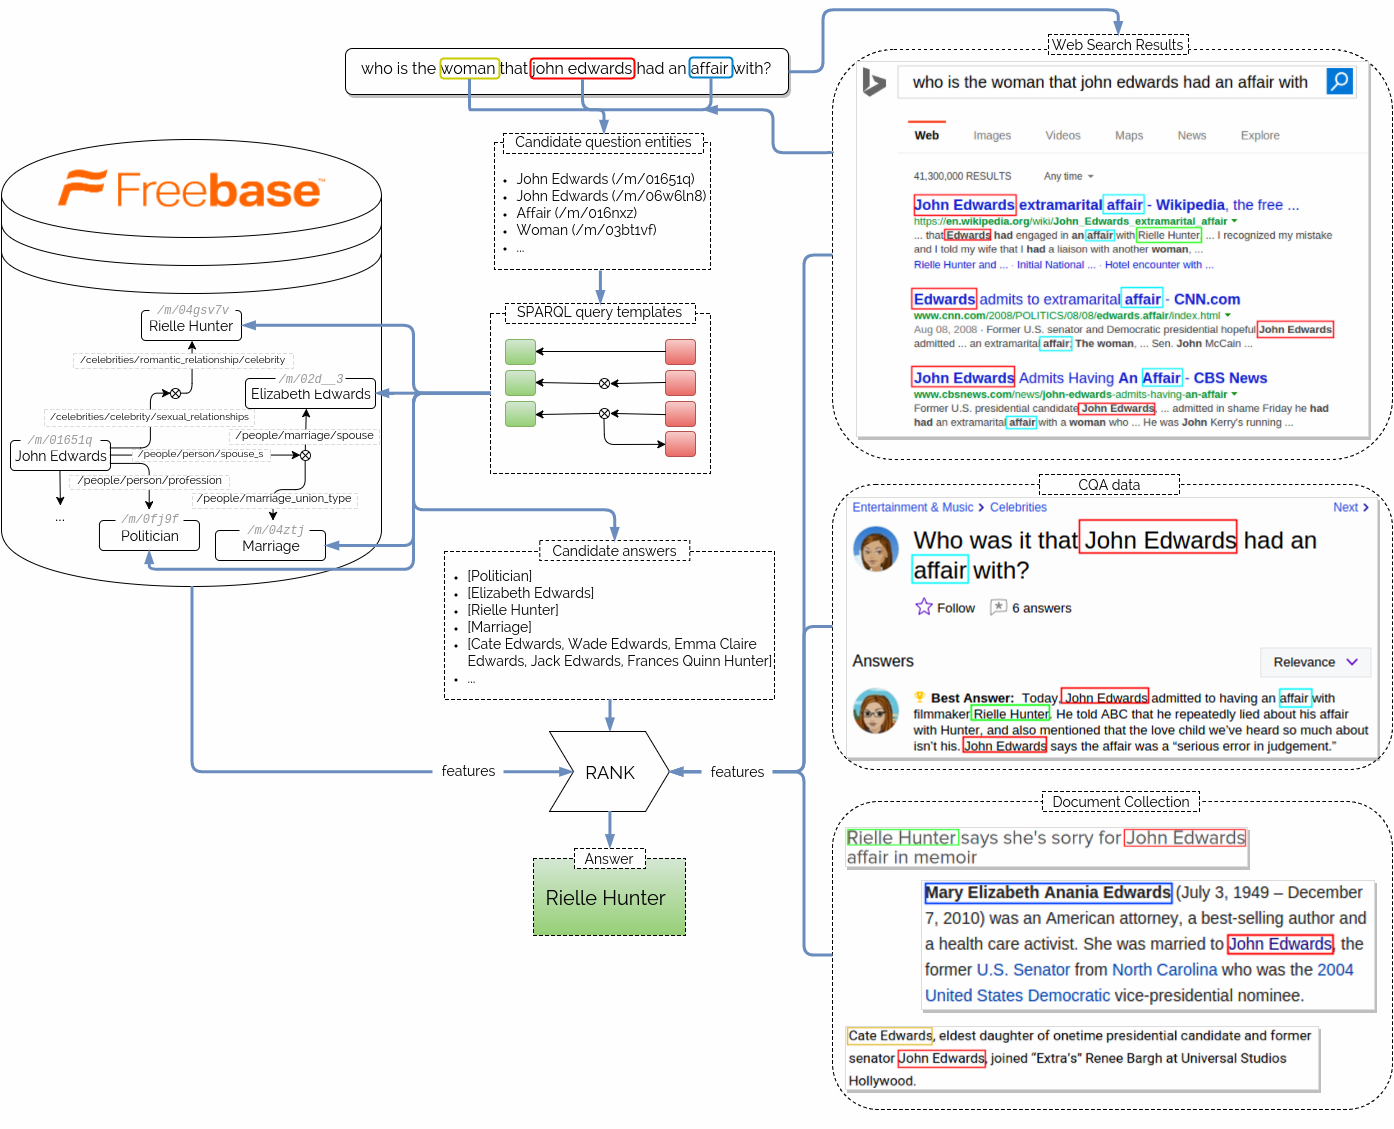
\includegraphics[width=0.9\textwidth]{img/Text2KB_model}
\vspace{-4mm}
\caption{The architecture of our Text2KB Question Answering system}
\label{fig:model}
\vspace{-3mm}
\end{figure*}


\subsection{The Aqqu KBQA system}
\label{sec:baseline:aqqu}

First, the system identifies question entities, which are used as sources for the answer search process.
For concreteness, consider a question from the WebQuestions dataset \textit{``who is the woman that john edwards had an affair with?''}.
Here, the entity \texttt{John Edwards} with Freebase id \texttt{/m/01651q} is the main question entity.
However, Freebase contains millions of entities and it can be difficult to identify the topical ones (\eg entities \texttt{Woman} and \texttt{Affair} are also present in Freebase), or to disambiguate and choose between \texttt{John Edwards} a politician (\texttt{/m/01641q}), an American racing driver (\texttt{/m/06zs089}) and other people with the same name.
% There is even an entity with the name ``\texttt{had an affair with}''\footnote{http://www.freebase.com/m/0c0n01x}.
Aqqu considers all spans of question words under certain conditions on part of speech tags and uses an entity names lexicon \cite{SPITKOVSKY12.266} to map phrases to potential entities.
Most reported systems, including Aqqu, do not disambiguate entities at this stage, but rather keep a set of candidates along with some information about their popularities (\eg number of mentions in the collection), and mention scores $p(entity| mention\ text)$.

At the next stage, SPARQL query candidates are generated by exploring the neighborhood of the question topic entities using a predefined set of query templates.
Each query template has question entities, predicates and answer placeholders.
The majority of the answers in the WebQuestions dataset can be covered by just 3 templates (q\_entity - question entity, a\_entity - answer entity, cvt\_node - Freebase mediator node, which represent tuples with more than 2 arguments):
\\

\begin{lstlisting}[frame=single,basicstyle=\small]
SELECT DISTINCT ?a_entity {
   <q_entity> <predicate> ?a_entity .
}
\end{lstlisting}

\vspace{-0.25cm}
\begin{lstlisting}[frame=single,basicstyle=\small]
SELECT DISTINCT ?a_entity {
   <q_entity> <predicate_1> ?cvt_node .
   ?cvt_node <predicate_2> ?a_entity .
}
\end{lstlisting}

\vspace{-0.25cm}
\begin{lstlisting}[frame=single,basicstyle=\small]
SELECT DISTINCT ?a_entity {
   <q_entity_1> <predicate_1> ?cvt_node .
   ?cvt_node <predicate_2> <q_entity_2> .
   ?cvt_node <predicate_3> ?a_entity .
}
\end{lstlisting}

The first template retrieves a set of entities that are directly connected to the given question entity via a certain predicate.
The second template accounts for the presence of a mediator node, that groups together arguments of a multi-argument relation.
And the last template looks for cases, when a question also mentions another argument of a multi-argument relation, \eg \texttt{Captain Kirk} and \texttt{Star Trek} for the question \textit{``who played captain kirk in star trek movie?''}.

Each query candidate is represented with a set of features, that includes the scores for linked question entities, various scores for matching between question term n-grams and query predicates, the size of the results list, \etc
The final stage of the question answering process is filtering and ranking. %Most state of the art systems employ some form of a learning-to-rank (LTR) model, trained on part of the dataset.
The Aqqu system employs a pairwise learning-to-rank model, trained on part of the dataset.
For each pair of candidate answers Aqqu creates an instance, which contains 3 groups of features: features of the first, the second candidate in the pair and the differences between the corresponding features of the candidates. Specifically, a Random Forest model is used in the provided Aqqu implementation. 
A pair where the first candidate is better than the second belongs to class +1, and -1 otherwise.
To reduce the number of pairs for the final ranking, Aqqu includes a simplified linear filtering model, which is trained to detect incorrect answers with high precision. 

\subsection{Basic system extensions}
\label{sec:baseline:extensions}
Before introducing our text-based improvements, we describe some basic extensions to the original Aqqu system.
First, we noticed that since Aqqu does not use information about the answer entity Freebase types, in many cases it returns an answer that is incompatible with the question: \eg state instead of county \etc
Therefore, we trained a model to return a score which measures compatibility between the question and answer entities, based on the entity notable types and question uni- and bi-grams as features, similar to Aqqu's relations score model.
A second extension introduced a new date range query template, which helps solve cases like \textit{``what team did david beckham play for in 2011?''}, where we need to look at the ranges of dates to determine whether an answer candidate satisfies the question.

\begin{lstlisting}[frame=single,basicstyle=\small]
SELECT DISTINCT ?a_entity {
   <q_entity_1> <predicate_1> ?cvt_node .
   ?cvt_node <from_predicate> ?date_from .
   ?cvt_node <to_predicate> ?date_to .
   ?cvt_node <predicate_2> ?a_entity .
   FILTER ( <question_date> >= ?date_from AND
            <question_date> <= ?date_to )
}
\end{lstlisting}

